
%%%%%%%%%%%%%%%%%%%%%%% file typeinst.tex %%%%%%%%%%%%%%%%%%%%%%%%%
%
% This is the LaTeX source for the TDPTemplate using
% the LaTeX document class 'llncs.cls' Springer LNAI format
% used in the RoboCup Symposium submissions.
% http://www.springer.com/computer/lncs?SGWID=0-164-6-793341-0
%
% It may be used as a template for your own TDP - copy it
% to a new file with a new name and use it as the basis
% for your Team Description Paper
%
% NB: the document class 'llncs' has its own and detailed documentation, see
% ftp://ftp.springer.de/data/pubftp/pub/tex/latex/llncs/latex2e/llncsdoc.pdf
%
%%%%%%%%%%%%%%%%%%%%%%%%%%%%%%%%%%%%%%%%%%%%%%%%%%%%%%%%%%%%%%%%%%%

\documentclass[runningheads,a4paper]{llncs}
\usepackage{amssymb}
\setcounter{tocdepth}{3}
\usepackage{graphicx}
\usepackage{amssymb}
\usepackage[utf8]{inputenc}
\usepackage{url}
\usepackage{float}
\usepackage{amsmath}
\usepackage{graphicx}
\usepackage{wrapfig}
\usepackage{tabto}

\usepackage{lipsum}
\newcommand{\BnL}[1][1em]{ 
\includegraphics[width=#1]{images/bnl.jpg} }

\begin{document}

\title{Walking Machine 2017 Team Description Paper}

\author{Jeffrey Cousineau \and Maxime St-Pierre, Jonathan Fortin, Thierry Pouplier, Alexandre Doyle, Jimmy Poirier, Cassandra Lépine, Philippe La Madelaine, Samuel Otis, Redouane Laref, Louis-Charle Labarre, Francis Grégoire, Simon Landry, Aloïs Goudard-Bellissens, Lucas Maurice, Léonore Jean-François, Nicolas Nadeau, Daniel Sami, Alexandre Salconi-Denis, Quentin Bourret, Laureline Estivalet, Julien Côté }
\institute{École de Technologie Supérieure \\ 1100 rue Notre-Dame Ouest, Montreal, QC, H3C 1K3 \\
\texttt{http://walkingmachine.ca}}
\maketitle


%%%%%%%%%%%%%%%%%%%%%%%%%%%%%%%%%%%%%%%%%%%%%%%%%%%%%%%%%%%%%%%%%%%%%%%%%%%%%%%%%%%%

\begin{abstract}

This paper gives details about the RoboCup@Home league team Walking Machine, from ETS University in Montreal, Canada for the next competition in Nagoya, Japan, in July 2017. The robot from Walking Machine, named SARA for Système d’Assistance Robotique Autonome (in English, Automated Robotic Assistance System), is a robot entirely built by the student scientific club from ETS. The robot is used for flexible interaction with humans, navigation and mobile
object manipulation. This document shows the electrical, mechanical and software properties and functionalities of SARA. It specifically emphasises on human following, object and people recognition as well as navigation, manipulation and human-robot interaction.

\end{abstract}


%%%%%%%%%%%%%%%%%%%%%%%%%%%%%%%%%%%%%%%%%%%%%%%%%%%%%%%%%%%%%%%%%%%%%%%%%%%%%%%%%%%%

\section{Introduction}
Walking Machine’s team is a young team from Montreal, Quebec, in Canada. We have been preparing our robot for the last year in prevision of the Robocup@home. Our team qualified with our robot, SARA, in the innovative design competition of Quebec Engineering Competition (CQI 2016, Polytechnic University, Montreal, Canada). The team went in many competitions in the past like the Eurobot, but made the leap for the RoboCup in the last years. \\

SARA, our creation, was designed for polyvalent human-robot interaction as well as efficient navigation and object manipulation. SARA is mounted on four mecanum wheels powered by Roboteq drives, has one arm mimicking a normal human arm, and sensors for communication and navigation. Our team has developed knowledge in object and people detection/recognition, as well as navigation using a laser scanner, odometry on the wheels and a XTION camera. All of these parts are interfaced through the Robot Operating System (ROS). \\

The next section will discuss the hardware design of SARA. Perceptions and decision making will be respectively shown in sections 3 and 4.


\section{Background}
% We are Buy n Large. We have no competitors so no background is required.
\lipsum[1-3]

\section{Software Architecture}
\tab Our software architecture is based on ROS (Robot Operating System). This allows us to build complex software in a short amount of time. 

\section{Perception}

\tab This year one of our new feature for our perception is an object classifier based on TensorFlow. This new approach is faster than our old method but requires some careful preparation. Our classifier is capable of classifying almost all the object found in an ordinary household. \\

We upgrade our robot with a second camera, a kinect v2 from Microsoft. This camera enables better point clouds and also better skeleton mesh to detect people. \\

\section{Artificial Intelligence}
\tab From last year experience, we made some change to the human machine interface. \\

The first change was to implement a state machine to reduce the number of launch file. This change permits us to reduce the time to setup the robot between task. 



\section{Experiments and results}
\lipsum[15-20]

\section{Conclusions and future work}
\lipsum[21-24]

\section*{Bibliography}
Add your references here
%\bibliographystyle{unsrt}
%\bibliography{bibliography}

\newpage
\section*{Robot SARA Hardware Description}
% TODO Change picture and description
Specifications for robot SARA are as follows:

\begin{table}

\label{my-label}

\begin{tabular}{l|p{90mm}}
\hline
\rowcolor[HTML]{FFFFFF} 
\multicolumn{2}{c}{\cellcolor[HTML]{FFFFFF}\textbf{SARA}}                                                      \\ \hline
\rowcolor[HTML]{EAEFF6} 
\textbf{Base}               & Custom base with fully holonomic platform                                        \\
\rowcolor[HTML]{FFFFFF} 
\textbf{Right arm}          & 7 DoF custom arm made of Kinova motors                                           \\
\rowcolor[HTML]{EAEFF6} 
\textbf{Neck}               & Tilt and pan unit using two Dynamixel MX-64R servo actuator                      \\
\rowcolor[HTML]{FFFFFF} 
\textbf{Head}               & Custom head made of RGB neopixels leds and Asus Xtion Pro                        \\
\rowcolor[HTML]{EAEFF6} 
\textbf{Gripper}            & Robotiq 2 fingers 140mm                                                           \\
\rowcolor[HTML]{FFFFFF}
\textbf{Dimensions}         & \begin{tabular}[c]{@{}l@{}}Base : 0,61m. X 0,77m.\\ Height : 1,68m.\end{tabular} \\
\rowcolor[HTML]{EAEFF6} 
\textbf{Weight}             & $\sim$60kg                                                                      \\
\rowcolor[HTML]{FFFFFF} 
\textbf{Additional sensors} & Hokuyo UTM-30LX on base                                                          \\
\rowcolor[HTML]{EAEFF6} 
\textbf{Microphone}         & Rode microphone											                         \\
\rowcolor[HTML]{FFFFFF} 
\textbf{Batteries}          & 2x 20V Dewalt drill battery 5aH                                                 \\
\rowcolor[HTML]{EAEFF6} 
\textbf{Computer}           & 1x Lenovo p50 with 32GB RAM and nVidia Quadro M2000 4GB, 1x Raspberry Pi 3       \\ \hline
\end{tabular}
\caption{Robot's hardware description}
\end{table}
\begin{wrapfigure}[10]{r}{0.25\textwidth}
	\centering
	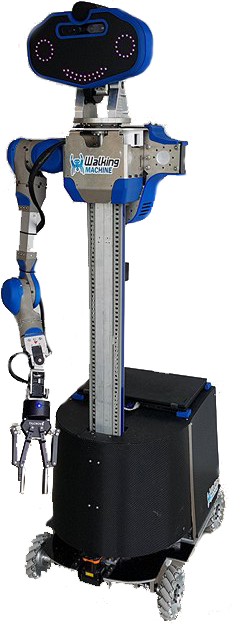
\includegraphics[width=0.30\textwidth]{images/sara_2.png}
	\caption{Robot SARA}
\end{wrapfigure}
\section*{Robot's Software Description}

For our robot we are using the following software:

\begin{itemize}
	\item Platform: Robotic Operating System (ROS) Kinetic on Ubuntu 16.04
	\item Navigation, localization and mapping: \href{http://wiki.ros.org/gmapping}{Gmapping}, \href{http://wiki.ros.org/amcl}{AMCL}, \href{http://wiki.ros.org/pointcloud_to_laserscan}{pointcloud\_to\_laserscan}
	\item Face recognition: \href{http://wiki.ros.org/people}{People}
	\item Speech recognition: \href{https://github.com/WalkingMachine/lab_ros_speech_to_text}{Google Speech API}
	\item Speech comprehension: \href{http://sag.art.uniroma2.it/lu4r.html}{LU4R}, \href{https://github.com/WalkingMachine/lu4r_ros}{lu4r\_ros}
	\item Speech generation: \href{https://doc.ubuntu-fr.org/svoxpico}{Svoxpico}
	\item Object recognition: \href{https://github.com/WalkingMachine/wm_darknet}{Darknet with YOLO v2 }
	\item Arm control: \href{http://wiki.ros.org/moveit}{MoveIt} and \href{https://github.com/Kinovarobotics/kinova-ros}{Kinova API}
	\item Task executor: \href{http://wiki.ros.org/flexbe}{Flexbe} 
	\item World reprensentation: \href{http://github.com/walkingmachine/wonderland}{Wonderland}
\end{itemize}

\end{document} 
